\documentclass[18pt]{beamer}
\usepackage[utf8]{inputenc} % for the umlauts
\usepackage{subfigure}

\beamertemplatenavigationsymbolsempty
%% SLIDE FORMAT

% use 'beamerthemekit' for standard 4:3 ratio
% for widescreen slides (16:9), use 'beamerthemekitwide'

\usepackage{templates/beamerthemekit}
% \usepackage{templates/beamerthemekitwide}

\setcounter{tocdepth}{1}

%% TITLE PICTURE

% if a custom picture is to be used on the title page, copy it into the 'logos'
% directory, in the line below, replace 'mypicture' with the 
% filename (without extension) and uncomment the following line
% (picture proportions: 63 : 20 for standard, 169 : 40 for wide
% *.eps format if you use latex+dvips+ps2pdf, 
% *.jpg/*.png/*.pdf if you use pdflatex)

%\titleimage{mypicture}

%% TikZ INTEGRATION

% use these packages for PCM symbols and UML classes
% \usepackage{templates/tikzkit}
% \usepackage{templates/tikzuml}

% the presentation starts here

\usepackage{mathabx}
\usepackage{picture}
\usepackage[absolute,overlay]{textpos}
%\usepackage[texcoord,grid,gridunit=mm,gridcolor=red, subgridcolor=green]{eso-pic}
\setbeamercovered{invisible}
\setbeamertemplate{caption}{\raggedright\insertcaption\par}

\title[SWT1]{Softwaretechnik 1 - 2. Tutorium}
\subtitle{Tutorium 03}
\author{Felix Bachmann}
\date{29.05.2017}

\institute{KIT - Institut für Programmstrukturen und Datenorganisation (IPD)}

% Bibliography

\usepackage[citestyle=authoryear,bibstyle=numeric,hyperref,backend=biber]{biblatex}
\addbibresource{templates/example.bib}
\bibhang1em

\begin{document}

% change the following line to "ngerman" for German style date and logos
\selectlanguage{ngerman}

%title page
\begin{frame}
\titlepage
\end{frame}

\begin{frame}
\tableofcontents
\end{frame}


\section{Orga}
	\subsection{Feedback 2. Übungsblatt}
	\begin{frame}
		\frametitle{2. Übungsblatt Statistik}
		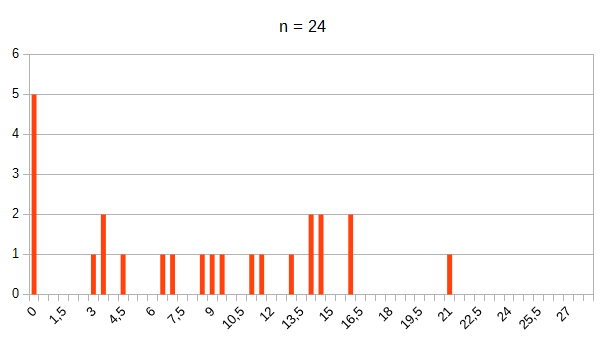
\includegraphics[scale=0.7]{./pics/tut2/statistics-ub2.png}
		\linebreak \centering $\diameter$ 8,35 bzw. 11,79 von 25 (28)
	\end{frame}

	
	\subsection{2. Übungsblatt - Fehler (Allgemein)}
	\begin{frame}
		\frametitle{Häufige Fehler}
		\begin{block}{Allgemein}
			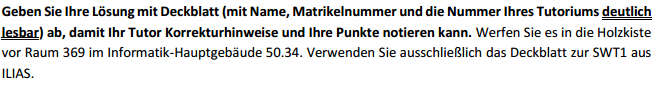
\includegraphics[scale=0.6]{./pics/tut2/deckblatt.png}
			\begin{itemize}
				\item $\implies$ nur das offizielle Deckblatt verwenden! (ab nächstes Mal Abzug)
				\pause
				\item häufigster Fehler: Aufgaben nicht abgegeben
			\end{itemize}
		\end{block}
	\end{frame}
	
	\subsection{2. Übungsblatt - Fehler}
	\begin{frame}
		\frametitle{Häufige Fehler}
		\begin{block}{Aufgabe 1 (Lastenheft): $\diameter$ 2,38 bzw. 3,56 von 5}
			\begin{itemize}
				\item Unnötiges aus Vorlage durfte man löschen (z.B. "'Siehe https://en.wikibooks.org/wiki/LaTeX/Glossary"' oder "'Szenarien"')
				\pause
				\item Anwendungsfälle beschreiben, was man in dem System tun kann 
				\linebreak $\implies$ beinhalten immer Verben! (z.B. "'Hobbyfotograph"' oder "'JMJRST"' ist kein Anwendungsfall)
			\end{itemize}
		\end{block}
	\end{frame}

	\begin{frame}
		\frametitle{Häufige Fehler}
		\begin{block}{Aufgabe 2 (Klassendiagramm): $\diameter$ 2,54 bzw. 4,07 von 8}
			\begin{itemize}
				\item oft wurden abstrakte Klassen "'Maler-Filter"' und "'Kunst-Filter"' vergessen
				\pause
				\item es wurden Dinge ergänzt, die so nicht explizit im Text standen
				\pause
				\item Ausrichtung des Bildes wurde nicht als Enum modelliert
				\pause
				\item falsche UML-Syntax (insb. Methode, Attribute)
			\end{itemize}
		\end{block}
	\end{frame}

	\begin{frame}
		\frametitle{Häufige Fehler}
		\begin{block}{Aufgabe 3 (Durchführbarkeitsanalyse): $\diameter$ 0,81 bzw. 1,95 von 3}
			\begin{itemize}
				\item sehr häufig nicht abgegeben
				\pause
				\item Fragen beantworten, nicht stellen!
				\linebreak z.B. "'Es werden 3 Java-Entwickler benötigt."' ergänzen durch
				"'Da wir 5 zur Zeit untätige Java-Entwickler in der Firma haben, ist das Projekt aus personeller Sicht für die Pear Corp. durchführbar."'
			\end{itemize}
		\end{block}
	\end{frame}

	\begin{frame}
		\frametitle{Häufige Fehler}
		\begin{block}{Aufgabe 4 (Geometrify programmieren): $\diameter$ 2,31 bzw. 5,05 von 10}
			\begin{itemize}
				\item NullPointerExceptions wurden geworfen  \linebreak
				$\implies$ deswegen sollte man seine eigene Lösung testen
				\pause 
				\item Java-Koordinaten != "'normale"' Koordinaten
				\pause
				\item Alpha-Kanal nicht beachtet
			\end{itemize}
		\end{block}
	
	\begin{block}{Aufgabe 5 (Kommandozeilen-Tool): $\diameter$ 0,31 bzw. 1,88 von 2}
		\begin{itemize}
			\item 4 Abgaben \dots
		\end{itemize}
	\end{block}
\end{frame}


\section{Zustandsdiagramm}
	\subsection{Intro(1)}
	\begin{frame}
		\frametitle{Wo sind wir? Pflichtenheft!}
		\begin{enumerate}
			\item Zielbestimmung  
			\item Produkteinsatz 
			\item Produktumgebung
			\item Funktionale Anforderungen 
			\item Produktdaten 
			\item Nichtfunktionale Anforderungen 
			\item Globale Testfälle
			\item Systemmodelle
			\begin{itemize}
				\item Szenarien
				\item Anwendungsfälle
				\item Objektmodelle $\implies$ UML-Klassendiagramme (letztes mal)
				\item \underline{\textbf{Dynamische Modelle}}
				\begin{itemize}
					\item UML-Zustandsdiagramm
					\item UML-Aktivitätsdiagramm
					\item UML-Sequenzdiagramm
					\makebox(0,0){\put(0,3.3\normalbaselineskip){%
							$\left.\rule{0pt}{1.5\normalbaselineskip}\right\}$ Heute!}}
				\end{itemize}
				\item Benutzerschnittstelle$\implies$ Zeichnungen/Screenshots
			\end{itemize}
			\item Glossar 
		\end{enumerate}
	\end{frame}

	\subsection{Intro(2)}
	\begin{frame}
		\frametitle{Begriffsklärung}
		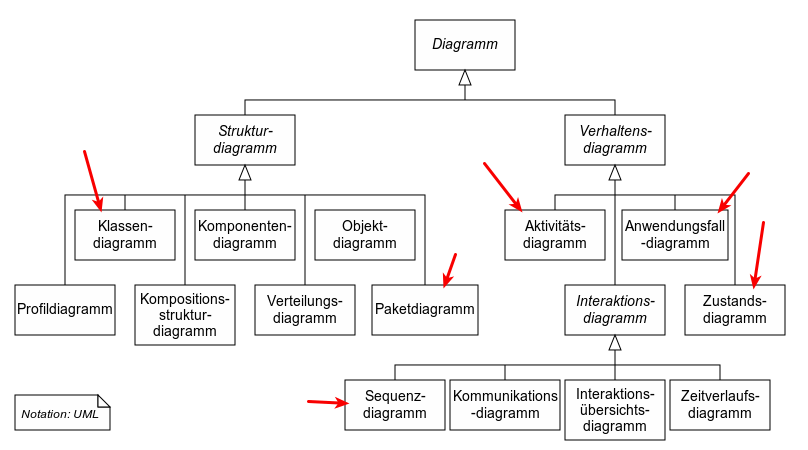
\includegraphics[scale=0.35]{./pics/tut1/uml_diagrams.png}
	\end{frame}

	\subsection{ZD: Allgemein}
	\begin{frame}
		\frametitle{Zustandsdiagramm - Allgemein}
		\begin{block}{Wozu braucht man das?}
			\pause
			\begin{itemize}
				\item Zustand \textbf{eines Objektes} beschreiben
				\item Zustandsüberführungsfunktion?
			\end{itemize}
		\end{block}
	\end{frame}

	\subsection{ZD: Allgemein (2)}
	\begin{frame}
		\frametitle{Zustandsdiagramm $\approx$ endlicher Automat}
		\begin{figure}
			\subfigure[GBI: DEA]{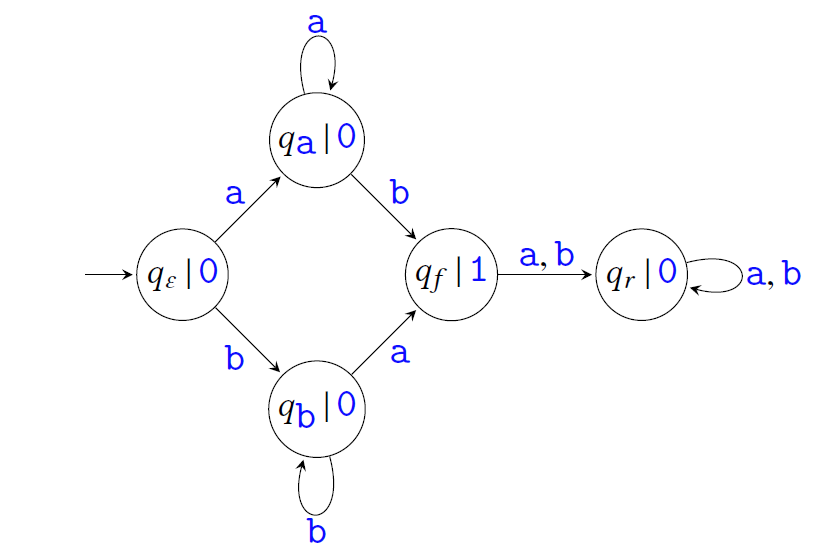
\includegraphics[scale=0.23]{./pics/tut2/auto_gbi.png}}
			\subfigure[SWT: Zustandsdiagramm]{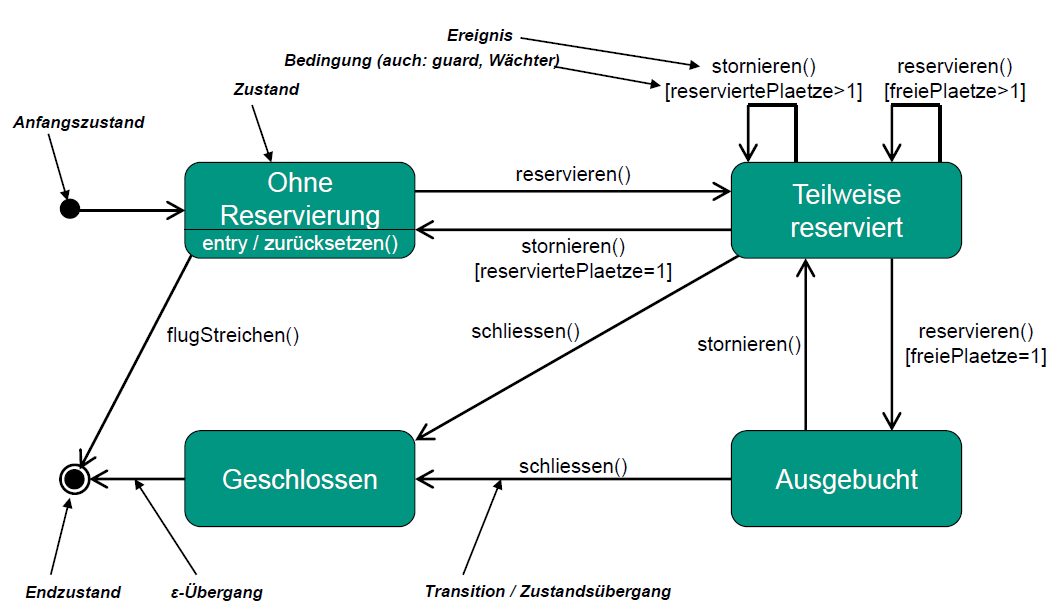
\includegraphics[scale=0.2]{./pics/tut2/auto_swt.png}}
		\end{figure}
	\end{frame}

	\subsection{ZD: Syntax(1)}
	\begin{frame}
		\frametitle{Zustandsdiagramm: Syntax}
		\begin{figure}
			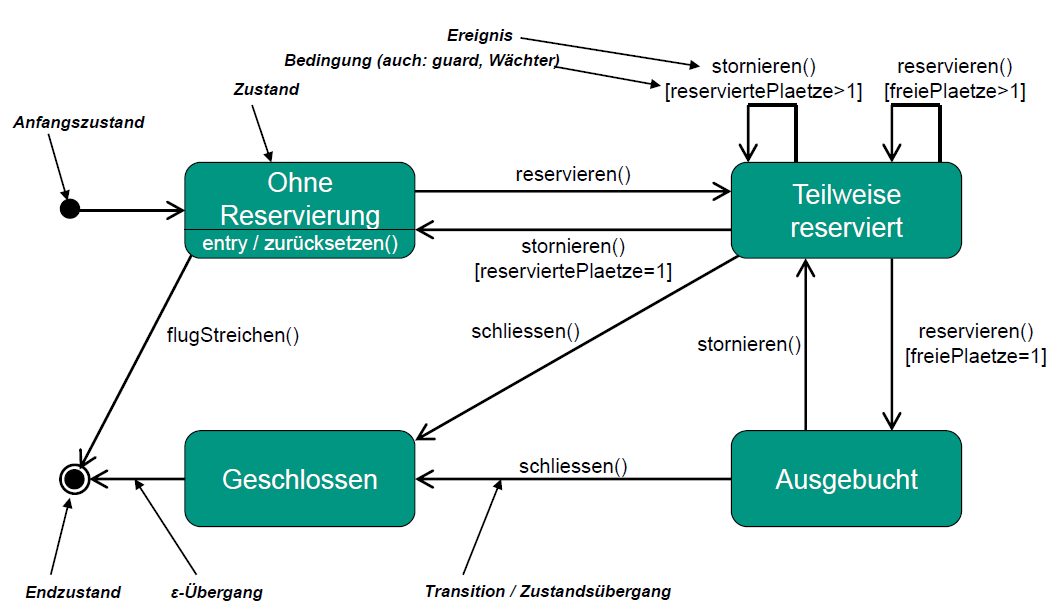
\includegraphics[scale=0.4]{./pics/tut2/auto_swt.png}
		\end{figure}	
	\end{frame}

	\subsection{ZD: Syntax (2)}
	\begin{frame}
		\frametitle{Zustandsdiagramm: Hierarchie}
		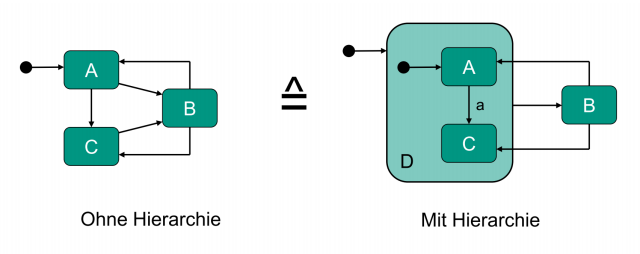
\includegraphics[scale=0.7]{./pics/tut2/auto_hier.png}	
	\end{frame}

	\subsection{ZD: Syntax (3)}
	\begin{frame}
		\frametitle{Zustandsdiagramm: Hierarchie - History}
		\begin{itemize}
			\item  History-Element, damit sich Hierarchie den letzten Zustand merkt
		\end{itemize}
		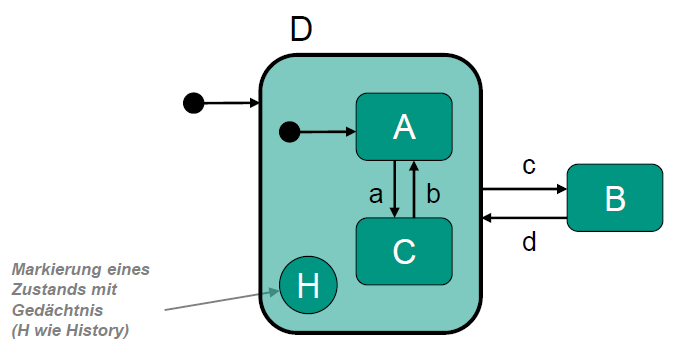
\includegraphics[scale=0.5]{./pics/tut2/auto_hier-hist.png}	
	\end{frame}

	\subsection{ZD: Syntax(4)}
	\begin{frame}
		\frametitle{Zustandsdiagramm: Nebenläufigkeit}	
		\begin{itemize}
			\item  mehrere Zustandsdiagramme in einem
		\end{itemize}
		\centering
		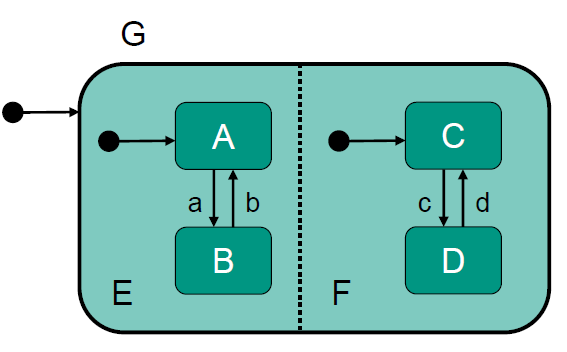
\includegraphics[scale=0.5]{./pics/tut2/auto_par.png}	
	\end{frame}

	\subsection{ZD: Aufgabe}
	\begin{frame}
		\frametitle{Klausuraufgabe SS09}
		Gegeben ist der folgende UML-Zustandsautomat. Geben Sie an, in welcher Zustandskombination
		sich der Zustandsautomat, jeweils ausgehend vom Startzustand, nach den beiden Eingabefolgen
		befindet.
		\centering
		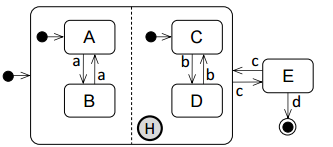
\includegraphics[scale=0.7]{./pics/tut2/auto_ex.png}
		\begin{itemize}
			\item a, b, c, c \pause $\implies$ AxD
			\item c, c, a, b, b, a, c, c, a \pause $\implies$ BxC
		\end{itemize}
	\end{frame}
		
\section{Aktivitätsdiagramm}
	\subsection{AD: Allgemein(1)}
	\begin{frame}
		\frametitle{Aktivitätsdiagramm - Allgemein}
		\begin{block}{Wozu braucht man das?}
			\pause
			\begin{itemize}
				\item Ablaufbeschreibungen (Kontrollfluss, Objektfluss)
				\item i.A. \textbf{mehrere verschiedene} Objekte
			\end{itemize}
		\end{block}
	\end{frame}

	\subsection{AD: Allgemein(2)}
	\begin{frame}
		\frametitle{Aktivitätsdiagramm - Beispiel}
		\begin{itemize}
			\item ist ebenfalls nicht neues!
		\end{itemize}
		\centering
		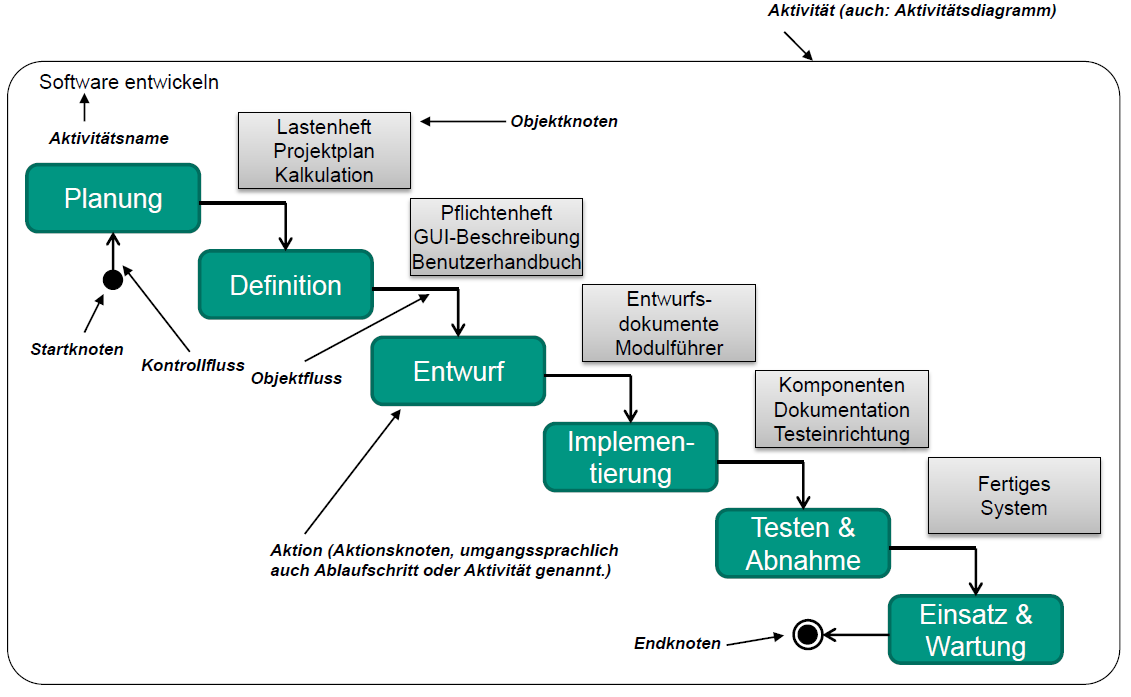
\includegraphics[scale=0.35]{./pics/tut2/act_wat.png}
	\end{frame}

	\subsection{AD: Syntax(1)}
	\begin{frame}
		\frametitle{Aktivitätsdiagramm - Syntax}
		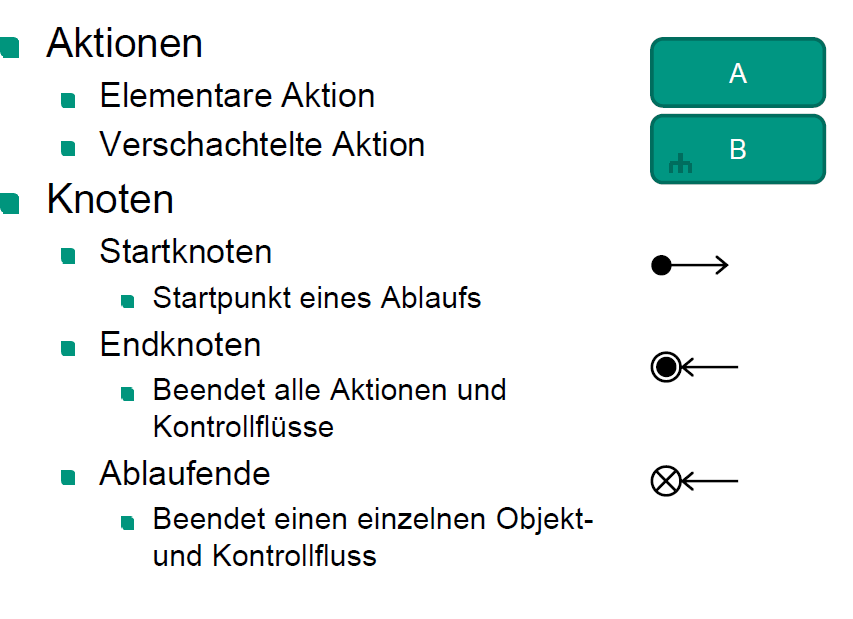
\includegraphics[scale=0.45]{./pics/tut2/act_syn1.png}
	\end{frame}

	\subsection{AD: Syntax(2)}
	\begin{frame}
		\frametitle{Aktivitätsdiagramm - Syntax}
		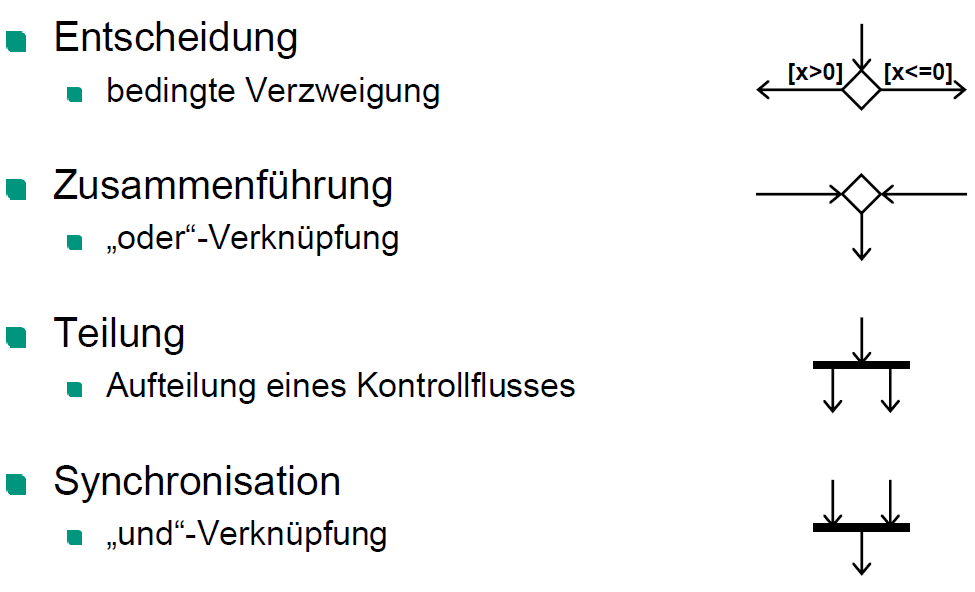
\includegraphics[scale=0.45]{./pics/tut2/act_syn2.png}
	\end{frame}

	\subsection{AD: Syntax(3)}
	\begin{frame}
		\frametitle{Aktivitätsdiagramm - Syntax}
		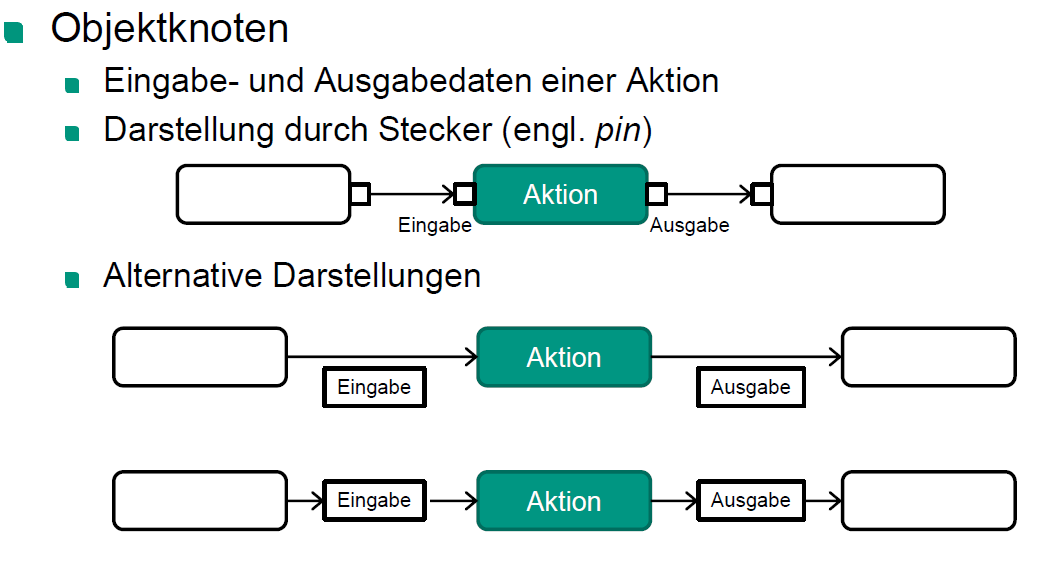
\includegraphics[scale=0.45]{./pics/tut2/act_syn3.png}
	\end{frame}

	\subsection{AD: Ablauf}
	\begin{frame}
		\frametitle{Aktivitätsdiagramm - Ablauf}
		\begin{itemize}
			\item Start am Startknoten mit einer Marke
			\item Aktionen werden erst ausgeführt, wenn an jedem Eingang eine Marke anliegt
			\item wurde eine Aktion ausgeführt, erscheinen an all ihren Ausgängen Marken
		\end{itemize}
	\end{frame}

	\subsection{AD: Beispiel}
	\begin{frame}
		\frametitle{Aktivitätsdiagramm - Beispiel}
		\begin{figure}
			\centering
			\caption{Wie kommt man hier zum Endknoten?}
			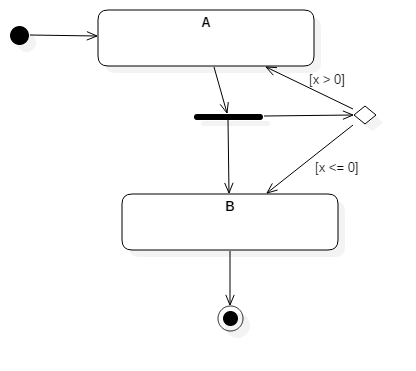
\includegraphics[scale=0.4]{./pics/tut2/act_ex.png}
		\end{figure}
	\end{frame}

\section{Sequenzdiagramm}
	\subsection{SD: Allgemein}
	\begin{frame}
		\frametitle{Sequenzdiagramm - Allgemein}
		\begin{block}{Wozu braucht man das?}
			\pause
			\begin{itemize}
				\item stellt den möglichen Ablauf eines Anwendungsfalls dar
				\item \textbf{zeitlicher Verlauf} von Methodenaufrufen, Objekterstellung, Objektzerstörung
			\end{itemize}
		\end{block}
	\end{frame}

	\subsection{SD: Syntax(1)}
	\begin{frame}
		\frametitle{Sequenzdiagramm - Syntax}
		\begin{itemize}
			\item Zeit verläuft von oben nach unten
			\item Lebenslinie
			\begin{itemize}
				\item gestrichelte senkrechte Linie
				\item eine pro Objekt
			\end{itemize}
			\item Steuerungsfokus
			\begin{itemize}
				\item dicker Balken über Lebenslinie
				\item zeigt, dass Objekt gerade aktiv ist
			\end{itemize}
			\item Nachrichtentypen
			\begin{itemize}
				\item Synchrone Nachricht (blockierend)
				\item Antwort (optional)
				\item Asynchrone Nachricht
			\end{itemize}
			\begin{textblock*}{20mm}(75mm,60mm)
				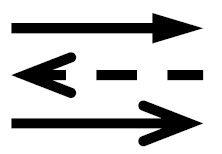
\includegraphics[scale=0.4]{./pics/tut2/sd_met.png}
			\end{textblock*}
		\end{itemize}
	\end{frame}

	\subsection{SD: Syntax(2)}
	\begin{frame}
		\frametitle{Sequenzdiagramm - Syntax}
			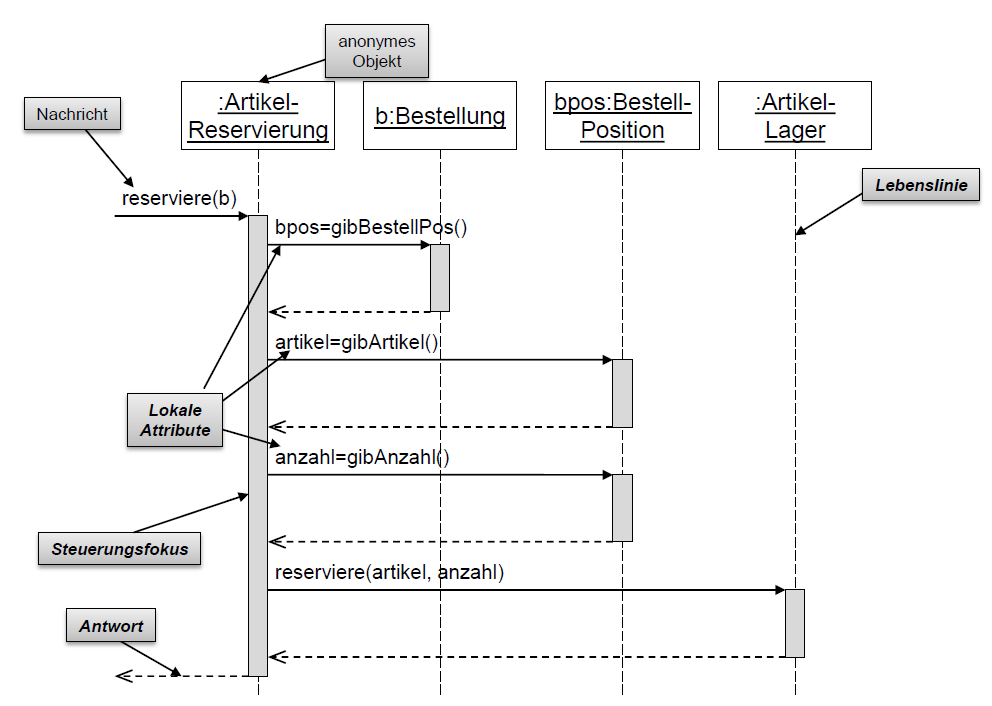
\includegraphics[scale=0.4]{./pics/tut2/sd_ex.png}
	\end{frame}

	\subsection{SD: Syntax(2)}
	\begin{frame}
		\frametitle{Sequenzdiagramm - Syntax}
		\begin{figure}
			\centering
			\subfigure[Objekt-Erzeugung]{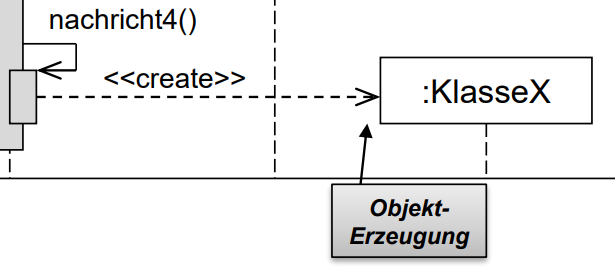
\includegraphics[scale=0.35]{./pics/tut2/sdcrea.png}}\newline
			\subfigure[Objekt-Zerstörung]{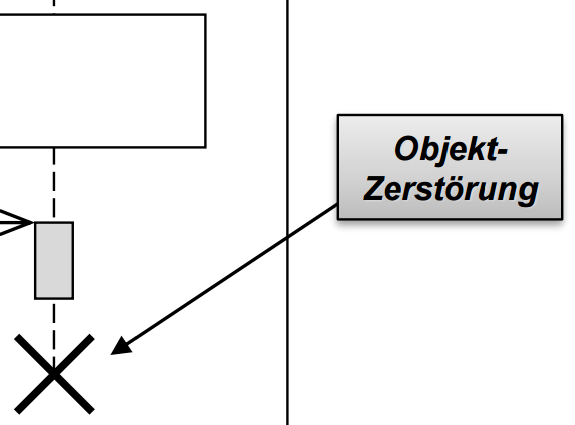
\includegraphics[scale=0.2]{./pics/tut2/sddestr.png}}
		\end{figure}
	\end{frame}

	\subsection{SD: Aufgabe}
	\begin{frame}
		\frametitle{Klausuraufgabe SS14}
			\begin{figure}
				\centering
				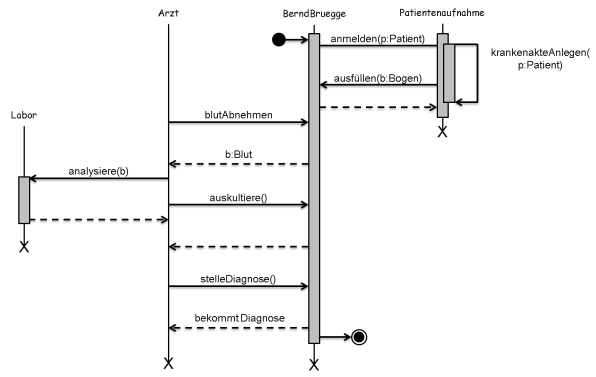
\includegraphics[scale=0.65]{./pics/tut2/sdtask.png}
				\caption{Hier stimmt was nicht\dots}
			\end{figure}
	\end{frame}

	\subsection{Gruppenarbeit}
	\begin{frame}
		\frametitle{Gruppenarbeit: Jetzt seid ihr dran!}
		Ablauf:
		\begin{enumerate}
			\item Einteilung in Expertengruppen
			\item Bearbeitet eure Aufgabe in der Gruppe
			\begin{itemize}
				\item Falls ihr Hilfe braucht, sagt Bescheid!
			\end{itemize}
			\item Vergleicht eure Lösung mit der Musterlösung 
			\item Durchmischen der Gruppen
			\item Stellt den anderen eure Aufgabe $\&$ Lösung vor
			\begin{itemize}
				\item Erklärt insbesondere, was ihr evtl. falsch gemacht habt
			\end{itemize}
		\end{enumerate}
	\end{frame}
	
	\subsection{Gruppe 1 - Aufgabe}
	\begin{frame}
		\frametitle{Gruppe 1: Zustandsdiagramm (Nachklausur 09)}
		\begin{tiny}
			Gegeben ist die folgende Beschreibung eines Automaten zum Verkauf von Getränken und
			Süßwaren: \linebreak
			\textit{Zu Beginn wartet der Automat auf die Auswahl des Produktes durch den Kunden. Die
			Produktauswahl findet in zwei Schritten statt. Zunächst wählt der Kunde die Ebene, in
			welcher sich das gewünschte Produkt befindet. Wählt der Kunde eine Ebene aus, die
			nicht existiert, wartet der Automat weiter auf die Produktauswahl. Ist die Ebene gewählt,
			gibt der Kunde das Fach des gewünschten Produktes an. Ist das gewählte Produktfach
			ausverkauft, bricht der Automat den Kaufvorgang ab und wartet erneut auf
			die Produktauswahl. Nach erfolgreicher Produktauswahl wirft der Kunde so lange
			Münzen ein, bis der eingeworfene Betrag gleich oder größer dem Preis des ausgewählten
			Produktes ist. Solange der Kunde nicht ausreichend Geld in den Automaten eingeworfen
			hat, wartet der Automat auf den Einwurf des fehlenden Geldbetrages. Hat der
			Kunde ausreichend Geld eingeworfen, befördert der Automat das gewählte Produkt in
			den Ausgabeschacht. Danach entnimmt der Kunde das Produkt. Hat der Kunde genau
			so viel Geld eingeworfen, wie das Produkt kostet, wartet der Automat auf die nächste
			Produktauswahl. Hat der Kunde das Produkt entnommen und mehr Geld eingeworfen,
			als das ausgewählte Produkt kostet, so gibt der Automat das Rückgeld in den Ausgabeschacht
			aus. Nachdem der Kunde das Rückgeld entnommen hat, wartet der Automat
			wieder auf die nächste Produktauswahl.} \linebreak
			Modellieren Sie das Verhalten des Automaten wie im obigen Szenario beschrieben als UMLZustandsdiagramm.
			Geben Sie zu jedem Übergang das auslösende Ereignis sowie ggf. die
			notwendige Bedingungen an.
		\end{tiny}
	\end{frame}
	
	\subsection{Gruppe 1 - Lösung}
	\begin{frame}
		\frametitle{Gruppe 1: Musterlösung}
		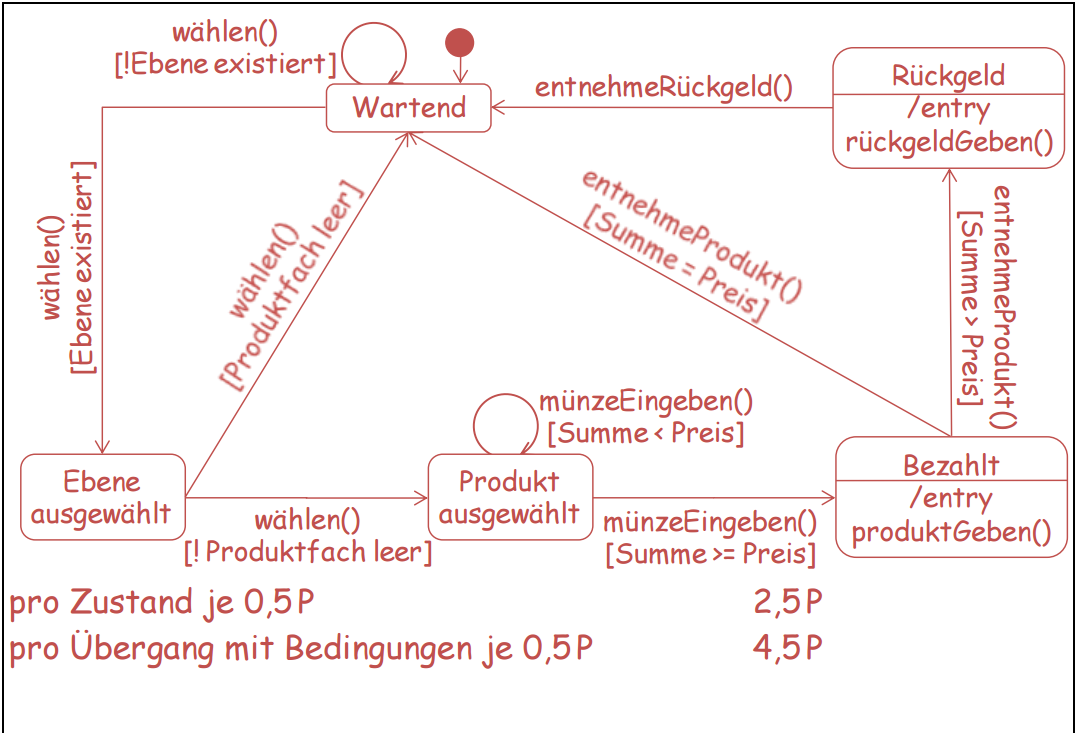
\includegraphics[scale=0.4]{./pics/tut2/group1sol.png}
	\end{frame}

	\subsection{Gruppe 2 - Aufgabe}
	\begin{frame}
		\frametitle{Gruppe 2: Sequenzdiagramm (Nachklausur 11)}
		\begin{tiny}
			Gegeben sei folgendes Szenario, welches eine Untersuchung in einem Krankenhaus beschreibt:  \linebreak
			\textit{Bernd Bruegge fühlt sich nicht wohl und möchte sich untersuchen lassen, um eine Diagnose
				zu erhalten. Er geht dazu ins Krankenhaus und meldet sich an der Patientenaufnahme
				an. Während der Sachbearbeiter an der Patientenaufnahme die Krankenakte anlegt,
				füllt Bernd B. den Anamnesebogen aus, den ihm der Sachbearbeiter gegeben hat.
				Nachdem Bernd B. den ausgefüllten Bogen dem Sachbearbeiter zurückgegeben hat, wird
				Bernd B. vom Arzt untersucht. Dazu nimmt er Bernd B. zunächst Blut ab. Während das
				Labor das Blut analysiert, führt der Arzt bei Bernd B. eine Auskultation durch. Schließlich
				bekommt Bernd B. vom Arzt seine Diagnose.} \linebreak
			Modellieren Sie das gegebene Szenario als UML-Sequenzdiagramm im Kasten auf der nächsten
			Seite (Querformat!). Verwenden Sie bei Ihrer Modellierung korrekte UML-Notation. Achten Sie
			bei Ihrer Modellierung darauf, auf welchen Objekten die Methoden sinnvollerweise aufgerufen
			werden müssen. Geben Sie ggf. Argumente der Methoden an. 
		\end{tiny}
	\end{frame}

	\subsection{Gruppe 2 - Lösung (1)}
	\begin{frame}
		\frametitle{Gruppe 2: Musterlösung}
		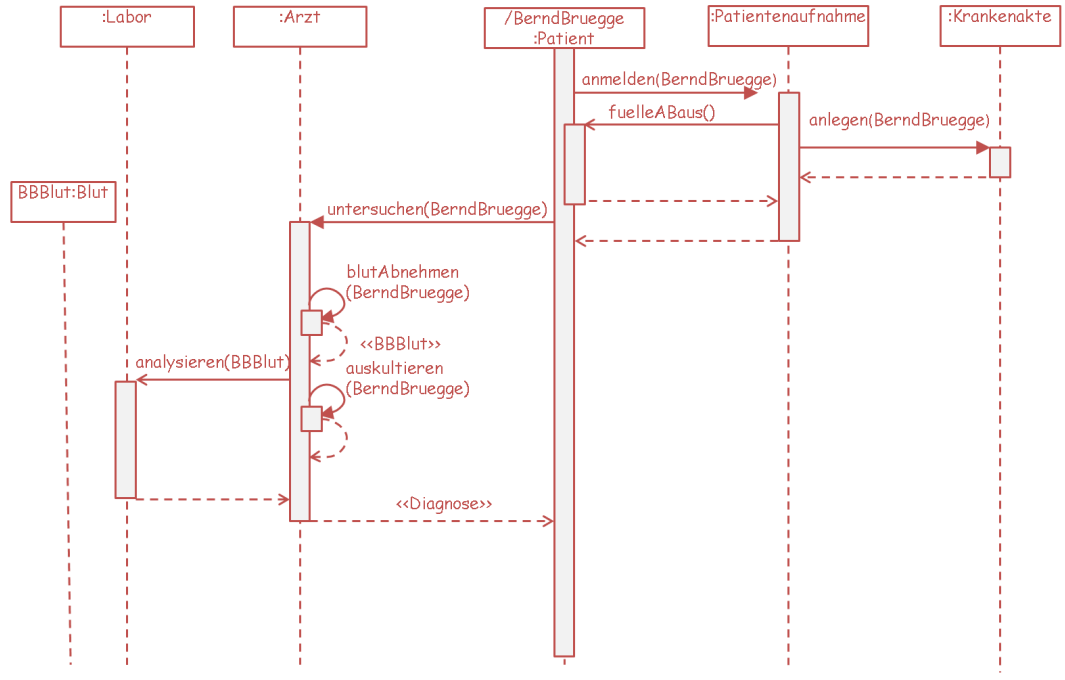
\includegraphics[scale=0.4]{./pics/tut2/group2sol1.png}
	\end{frame}

	\subsection{Gruppe 2 - Lösung(2)}
	\begin{frame}
		\frametitle{Gruppe 2: Musterlösung}
		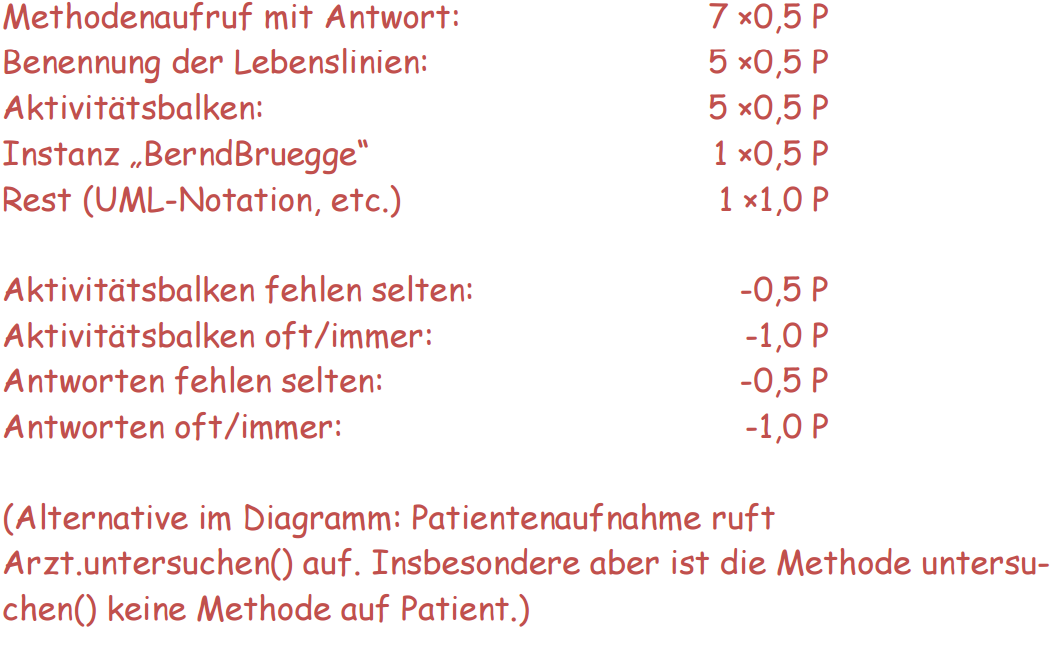
\includegraphics[scale=0.4]{./pics/tut2/group2sol2.png}
	\end{frame}

	\subsection{Gruppe 3 - Aufgabe}
	\begin{frame}
		\frametitle{Gruppe 3: Aktivitätsdiagramm (Hauptklausur 06)}
		\begin{tiny}
			Entwerfen Sie ein Aktivitätsdiagramm, das die Durchführung einer Klausur beschreibt. Halten
			Sie sich dabei so eng wie möglich an die nachfolgende Beschreibung und achten Sie darauf,
			parallele Aktivitäten korrekt zu synchronisieren. Beginnen Sie mit der Modellierung der
			Aktivitäten nach Betreten des Hörsaals.
			Hinweis: Aktivitäten der Studenten sind nicht zu modellieren.   \linebreak
			\textit{Nach Betreten des Hörsaals beginnt A1 die Tafel zu beschriften, während einer seiner
				Helfer die Etiketten auslegt und der andere die mitgebrachten Türschilder
				(„Bitte nicht stören! Klausur!“) an den Türen anbringt. Auf den Etiketten stehen
				der Vor- und Nachname jedes Studenten, seine Matrikelnummer und eine fortlaufende
				Nummer, die später die Verwaltung der Klausur vereinfacht.
				Sind diese Aufgaben erledigt, kann der Einlass beginnen. Dazu öffnen die Helfer
				die Türen des Hörsaals und A1 beaufsichtigt den Einlass. Solange noch nicht alle
				Studenten ihren Platz gefunden haben, helfen A2 und A3 bei der Platzsuche.
				Der Hauptverantwortliche A1 wartet ab, bis alle ihre Plätze gefunden haben. Dann
				erklärt er den Ablauf, beaufsichtigt das Austeilen der Klausurblätter und verkündet
				den Beginn der Klausur. Anschließend beaufsichtigt er 60 Minuten lang die Klausur
				und sagt das Ende der Klausur an.
				Nachdem A1 den Ablauf der Klausur angesagt hat, sind A2 und A3 für das Austeilen
				der Klausur, die anschließende Aufsicht zuständig. Während der Bearbeitungszeit
				geht zusätzlich einer von beiden herum und kontrolliert die Studentenausweise,
				während der andere Aufsicht führt.
				Während der Klausur verlässt keine Aufsicht den Hörsaal. } \linebreak
		\end{tiny}
	\end{frame}

	\subsection{Gruppe 3 - Lösung }
	\begin{frame}
	\frametitle{Gruppe 3: Musterlösung}
	\centering
	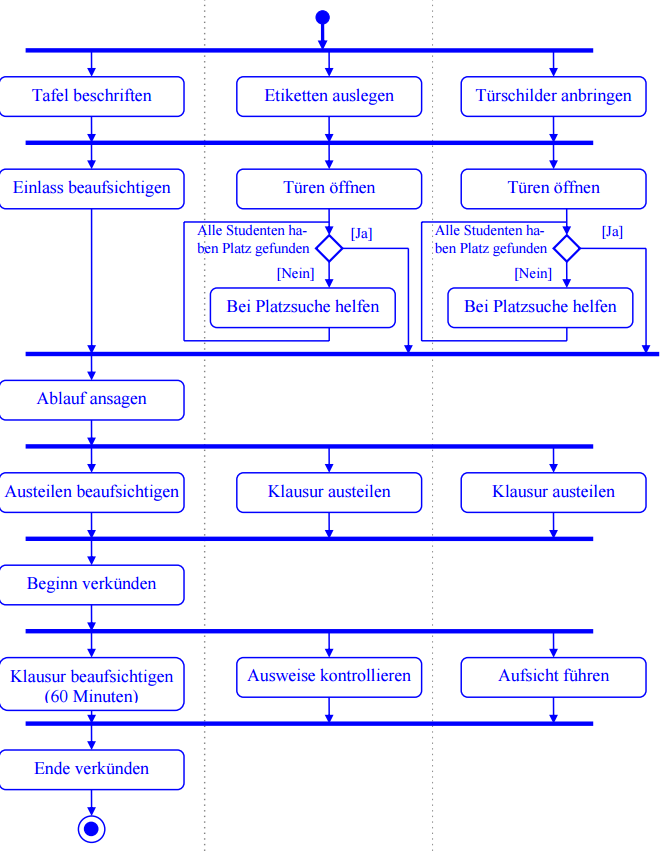
\includegraphics[scale=0.35]{./pics/tut2/group3sol.png}
	\end{frame}


\section{Tipps}
	\subsection{Tipps}
	\begin{frame}
		\frametitle{Tipps - 3. Übungsblatt}
			\begin{exampleblock}{Aufgabe 1-3: Plug-In programmieren}
				\begin{itemize}
					\pause
					\item JavaDoc + CheckStyle \dots
					\item Fügt junit in die jeweilige Untermodul-pom ein
					\item Java Swing benutzen (schaut euch die Java-Klassen JMenu und JMenuItem an)
				\end{itemize}
			\end{exampleblock}
			\pause
			\begin{exampleblock}{Aufgabe 4: Aktivitätsdiagramm}
				\begin{itemize}
					\pause 
					\item seperate Diagramme $\implies$ verschachtelte Aktionen
				\end{itemize}
			\end{exampleblock}
	\end{frame}

	\begin{frame}
		\frametitle{Tipps - 3. Übungsblatt}
			\begin{exampleblock}{Aufgabe 5: Sequenzdiagramm}
				\begin{itemize}
					\pause
					\item auf welchen Objekten/Klassen werden Methoden aufgerufen?
					\item auf Pfeile var=methode() schreiben, wenn Rückgabe von methode() in var gespeichert wird
				\end{itemize}
			\end{exampleblock}
			\pause
			\begin{exampleblock}{Aufgabe 6: Substitutionsprinzip}
				\begin{itemize}
					\pause
					\item Folien "'Folgerung aus dem Substitutionsprinzip"' anschauen (Ko-/Kontravarianz)
					\item mal als Java-Programm hinschreiben und versuchen zu kompilieren
				\end{itemize}
			\end{exampleblock}
	\end{frame}
	
	\subsection{Tichy}
	\begin{frame}
		\frametitle{Falls euch mal langweilig ist :D}
		\centering \url{www.tichy.click}
	\end{frame}
	
	\subsection{Abgabe}
	\begin{frame}
		\frametitle{Denkt dran!}
		\begin{alertblock}{Abgabe}
			\begin{itemize}
				\item Deadline am 7.6 um 12:00
				\item Aufgabe 4+5+6 handschriftlich (auf saubere Syntax achten!)
				\item an das Deckblatt denken!!
			\end{itemize}
		\end{alertblock}
	\end{frame}
		
	\begin{frame}
		\frametitle{Bis dann! (dann := 12.06.17)}
		\centering
		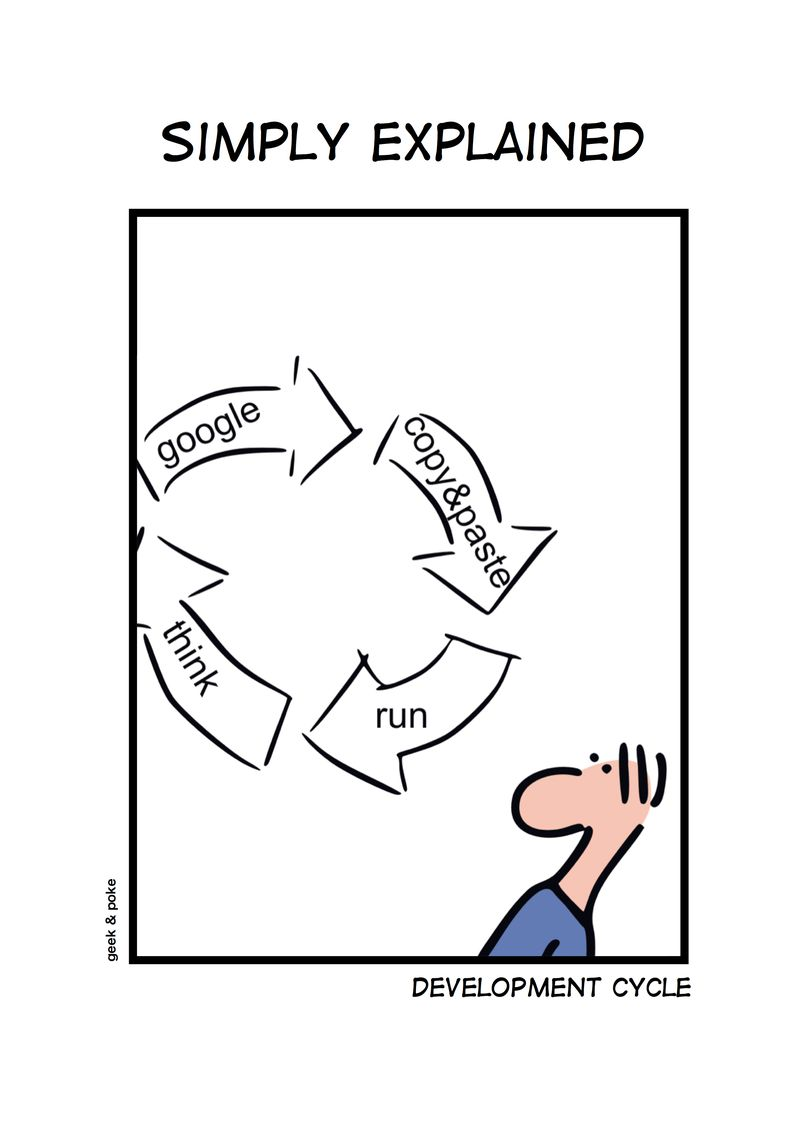
\includegraphics[scale=0.9]{./comics/geek_and_poke_development.jpg}
	\end{frame}

\end{document}
